%\epigraph{Yesterday's rose stands only in name, we hold only empty names.}{--- \textup{Umberto Eco}, \textit{The Name of Rose}}

In this chapter, I will give an overview of the neutrino and its properties. After an introduction of the history studies, two important properties: the flavor transformations and the neutrino mass are discussed. %The phenomenon, theories 

\section{Discovery of Neutrino}
The existence of neutrinos was first put forward by Wolfgang Pauli in the 1930s to solve the contradictions observed in beta decay experiments. It was shown definitively by James Chadwick in 1914 that the electrons emitted in beta decay did not have a discrete set of energies but instead had a continuous spectrum\cite{leite1996weak}. This means that the energy, momentum and angular momentum (spin) were not conserved between the nucleus and electron. To solve this problem, Wolfgang Pauli introduced a charge-neutral, spin-1/2 and nearly massless new particle. The sum of the energies of the new particle, the nucleus and electron is constant, which solved the problem. 

In 1934, Bethe and Peierls suggested direct neutrino detection via a neutrino-induced interaction, called the inverse beta decay (IBD): $\bar{\nu}_e+p\to e^+ + n$. Their calculation showed that the IBD cross section was of the order of $10^{-44}$ cm$^2$. Such a small cross section indicates that the neutrino is difficult to detect\cite{bethe1934neutrino}.

In 1956, Fred Reines and Clyde Cowan made the first discovery of the neutrino (specifically, it was electron antineutrinos $\bar{\nu}_e$) by using a nuclear reactor as an intense neutrino source with neutrino fluxes on the order of $10^{12}-10^{13}$ neutrinos/second/cm$^2$. The active volume of their detector was two tanks filled with water in which cadmium chloride (CdCl$_2$) was dissolved. The water tanks were surrounded by liquid scintillator layers coupled with photomultiplier tubes (PMT) to detect emitted photons. The incoming antineutrinos interacted with the water via IBD. The produced positrons quickly annihilated with $e^-$ and gave $\gamma$ signals while the produced neutrons went through the neutron capture process: $n+^{108}$Cd$\to^{109}$Cd$^*\to^{109}$Cd$+\gamma$ and gave delayed $\gamma$ signals. A coincidence of these two characteristic signals provided a distinctive signature for the neutrino reaction. They measured the cross-section as $6.3\times10^{-44}$ cm$^2$, which was consistent with Bethe's calculation\cite{reines1960detection}.

\section{Solar Neutrino: Early Studies}
In the 1930s, Hans Bethe et al. explained the origin of the Sun's energy as a series of nuclear reactions\cite{bethe1939energy}.

Based on the available physics and experimental data, the Standard Solar Model (SSM) is a modern accepted theory for the evolution of the Sun. The energy in the Sun is mainly produced by two sets of reactions: the proton-proton (pp) chain, which contributes to $\sim 98.6\%$ of the energy release and the Carbon-Nitrogen-Oxygen (CNO) cycle, which contributes $\sim 1.4\%$. Fig.~\ref{ppChain} and Fig.~\ref{CNOcycle} show all the reactions in the two sets respectively. Via these two main sets of nuclear reactions, hydrogen is eventually fused into helium, and the net nuclear transformation is: $4p+2e^-\to^{4}$He$+2\nu_e+Q$, where the released energy, $Q$ is 26.73 MeV. This energy release includes kinetic energy of particles as well as annihilation of positron and electrons in the solar plasma\cite{antonio2018state}.

The neutrinos produced in the solar nuclear reactions (the solar neutrinos) can be detected on the Earth\cite{giunti2007fundamentals}. Due to the branching ratios and unterminated chains in the pp chain and CNO cycle, the solar neutrinos come from different reactions, as shown in Table~\ref{solarnu}. The solar neutrinos detected on the Earth are named after the specific fusion process\cite{haxton2013solar}. They have different fluxes and energies, as shown in Fig.~\ref{bp05plot}\cite{bahcall2005new}.

\begin{figure}[htbp]
	\centering	
	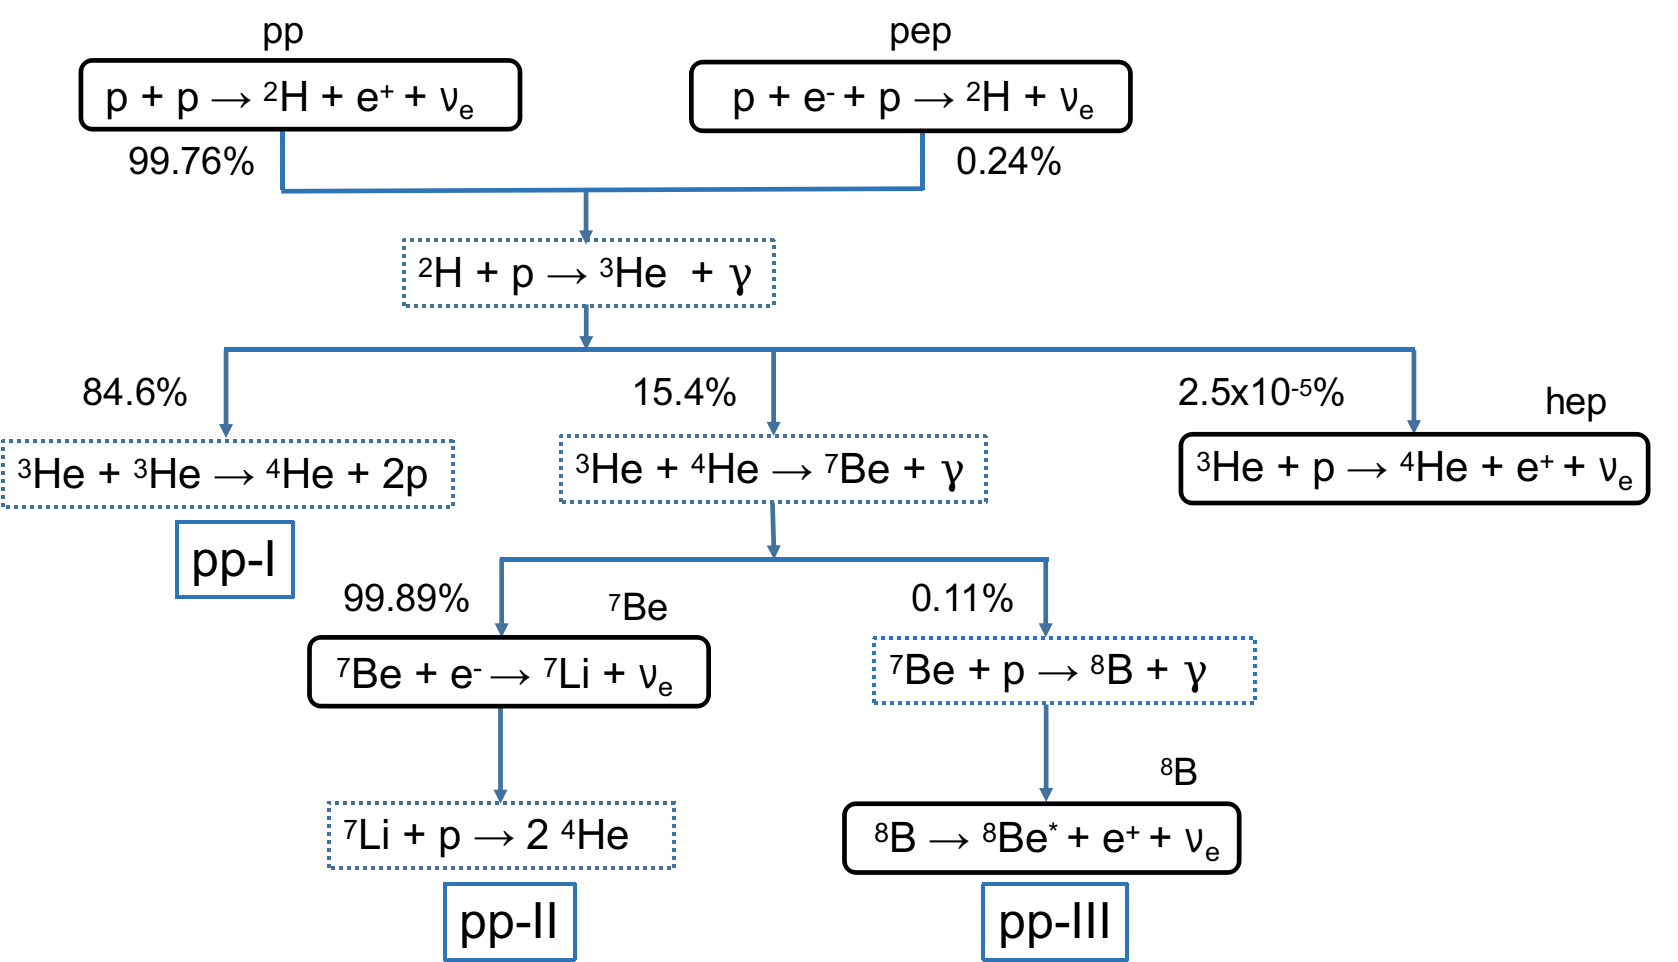
\includegraphics[width=14cm]{ppChain.png}
	\caption{All reactions in the three PP chains: PP-I, PP-II, PP-III. The reactions producing neutrinos are labeled in the solid frames. Modified from \cite{oberauer2020solar}.}
	\label{ppChain}
\end{figure}


\begin{figure}[htbp]
	\centering	
	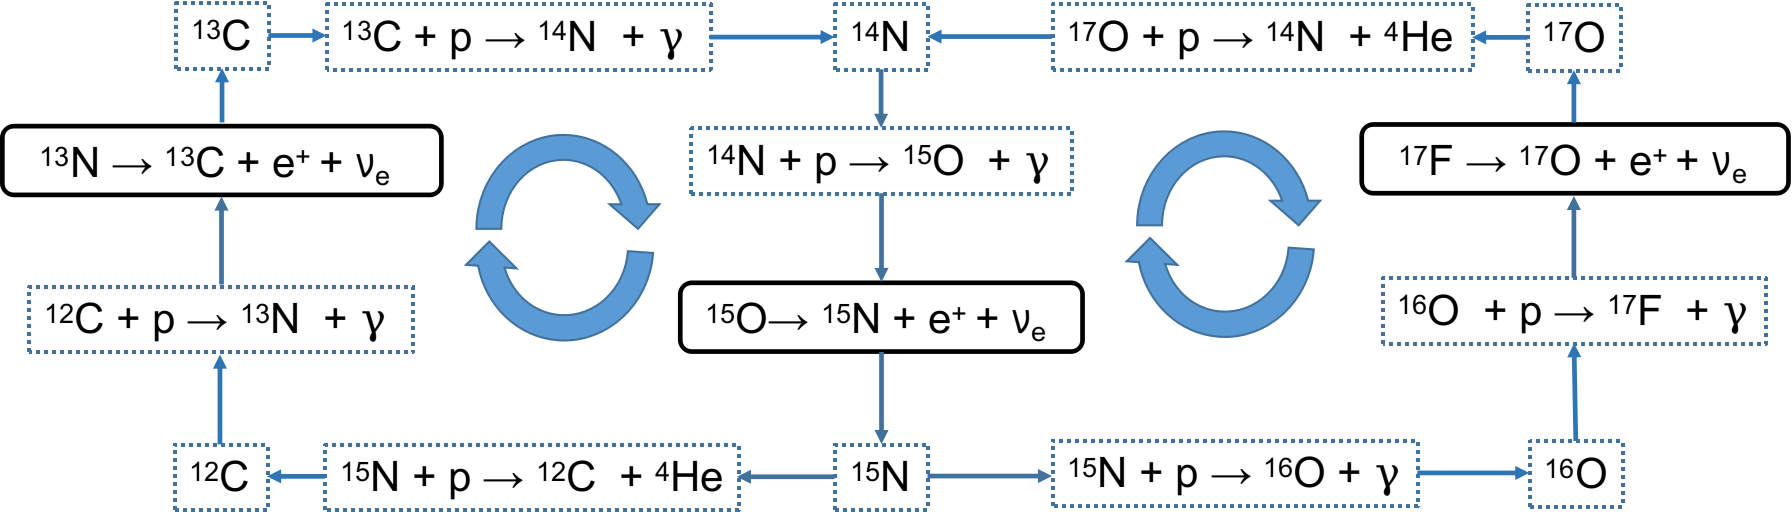
\includegraphics[width=14cm]{CNOcycle.png}
	\caption{All reactions in the CNO bicycle. The reactions producing neutrinos are labeled in the solid frames. Modified from \cite{oberauer2020solar}.}
	\label{CNOcycle}
\end{figure}

\begin{table}[htp]
	\caption[]{\label{solarnu} Solar neutrinos from reactions in pp chain (a) and CNO cycle (b).}	
	\subfigure[pp chain]{
		\begin{tabular*}{62mm}{cc}
			\toprule 
			solar $\nu_e$  & reaction  \\
			\midrule
			pp & $p+p\to ^2$H $+e^++\nu_e$ \\
			pep & $p+e^-+p\to^2$H $+~\nu_e$ \\
			hep &  $^3$He $+~p\to^4$He $+~e^++\nu_e$ \\ 
			$^7$Be &  $^7$Be $+~e^-\to^7$Li $+~\nu_e$\\
			$^8$B & $^8$B$\to^8$Be$^*+e^++\nu_e$\\
			\bottomrule	
		\end{tabular*}
	}
	\subfigure[CNO cycle]{
		\begin{tabular*}{60mm}{cc}
			\toprule 
			solar $\nu_e$   & reaction \\
			\midrule
			CNO &$^{13}$N$\to^{13}$C$+e^++\nu_e$\\	
			& $^{15}$O$\to^{15}$N$+e^++\nu_e$ \\
			& $^{17}$F$\to^{17}$O$+e^++\nu_e$ \\
			\bottomrule	
		\end{tabular*}
	}
\end{table}

\begin{figure}[htbp]
	\centering	
	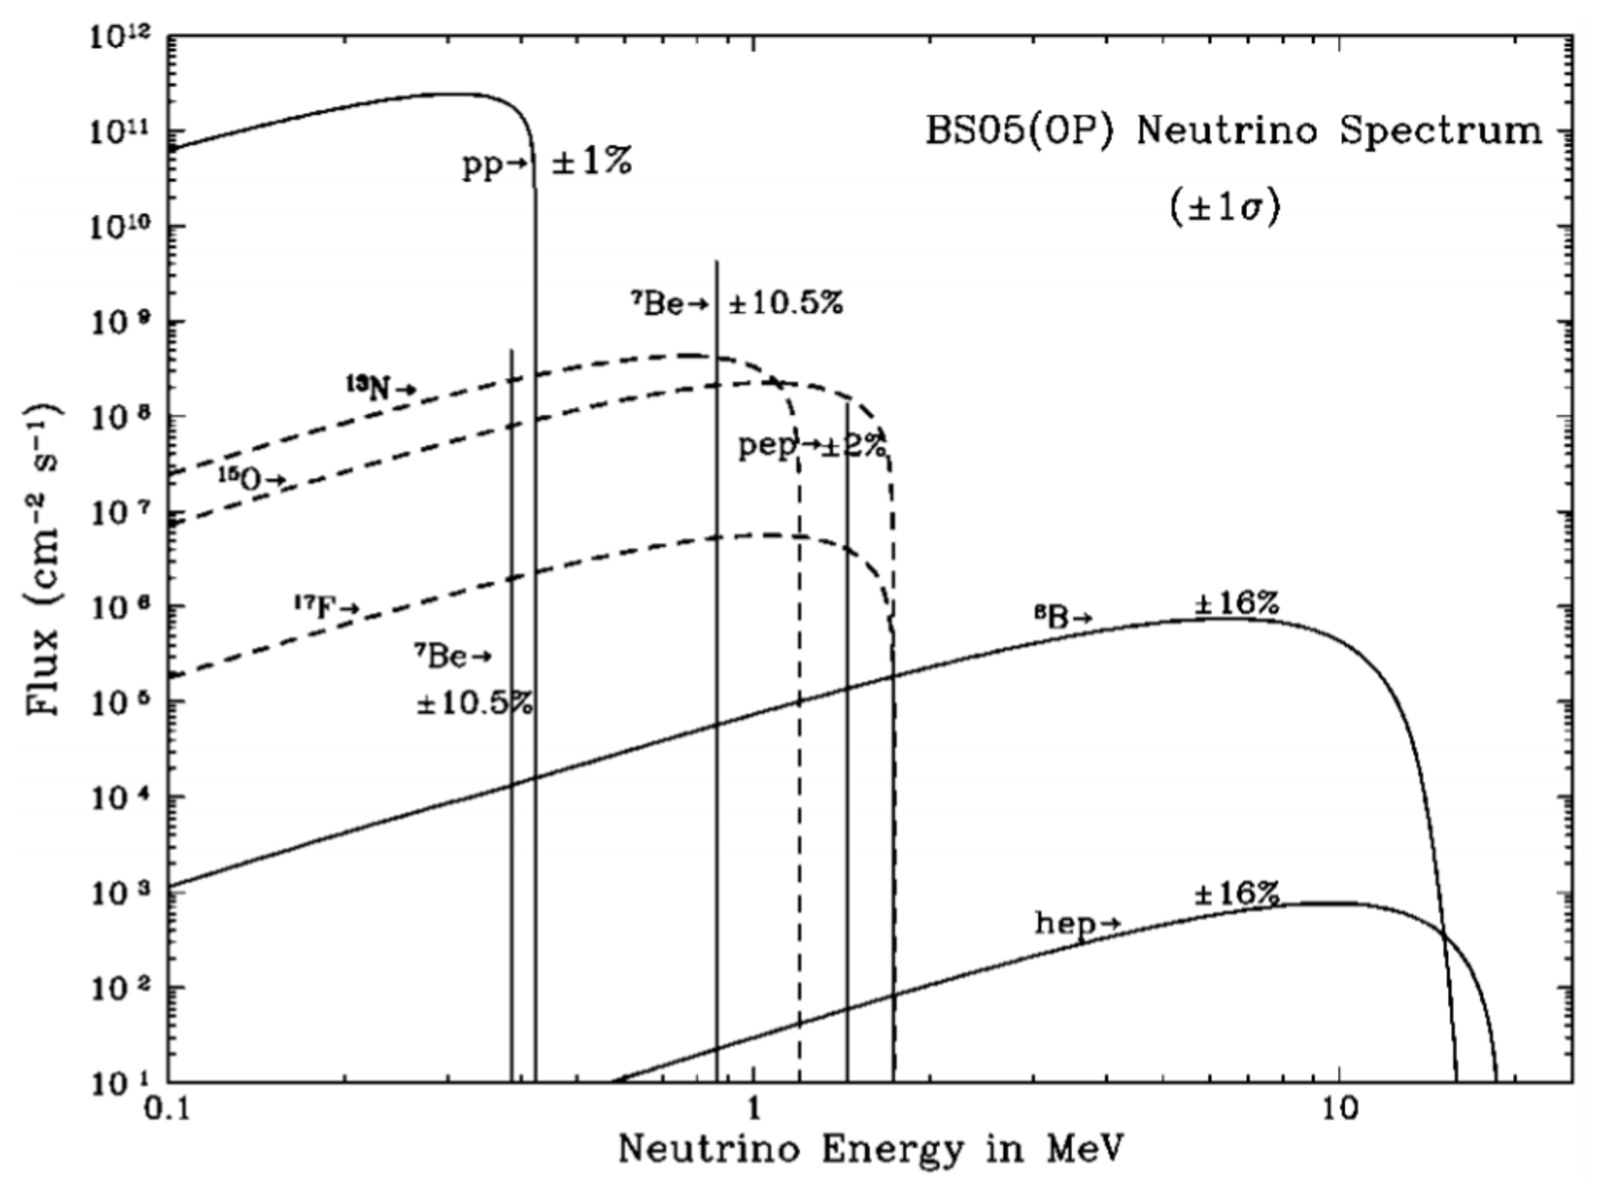
\includegraphics[width=10cm]{BP05.pdf}
	\caption{ Solar neutrino energy spectrum ($E_\nu$ vs. flux) for the solar model BS05(OP). Figure is from \cite{bahcall2005new}.}
	\label{bp05plot}
\end{figure}

%\subsection{Early Experiments}
In 1964, John Bahcall and Raymond Davis proposed the first experiment to detect solar neutrinos\cite{bahcall1964solar,davis1964solar}. Raymond Davis designed an experiment that used a 380 m$^3$ tank filled with Perchloroethylene (C$_2$Cl$_4$), a dry-cleaning fluid rich in chlorine. Solar neutrinos were expected to change $^{37}$C1 to $^{37}$Ar via the endothermic reaction $\nu_e+^{37}$Cl$\to^{37}$Ar$+e^-$ and the produced $^{37}$Ar were extracted and counted. The neutrino energy threshold ($E_{thresh}$) of the experiment was 0.814 MeV, which allowed a measurement mostly of the $^8$B neutrino flux but also including some lower energy neutrinos\cite{davis1964solar}. Their first results, announced in 1968, showed that only about one-third of the predicted radioactive argon atoms were measured. This raised a problem of missing solar neutrinos.


\begin{figure}[htbp]
	\centering
	\begin{minipage}[t]{0.45\textwidth}{(a)}
		\centering
		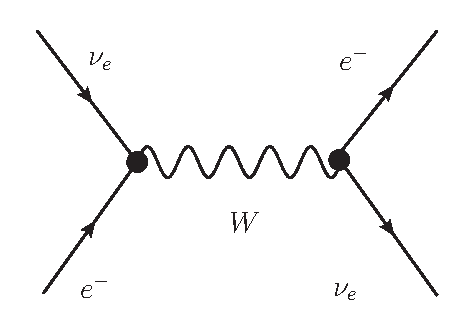
\includegraphics[width=4.5cm]{charged-1.eps}
	\end{minipage}
	\begin{minipage}[t]{0.3\textwidth}{(b)}
		\centering
		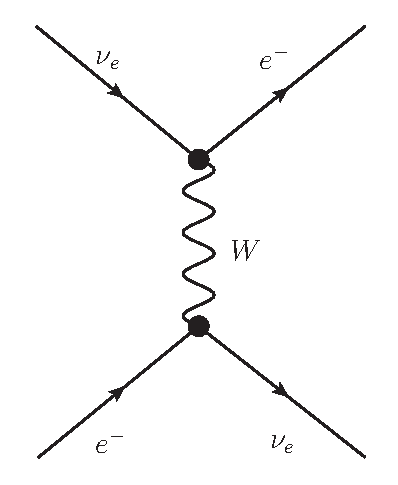
\includegraphics[height=4cm]{charged.eps}
	\end{minipage}
%	\begin{minipage}[t]{0.4\textwidth}{(c)}
%	\centering
%	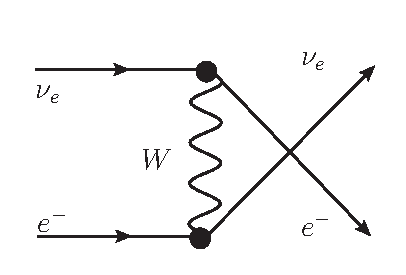
\includegraphics[width=4.5cm]{charged-u.eps}
%\end{minipage}
	\begin{minipage}[t]{0.4\textwidth}{(c)}
	\centering
	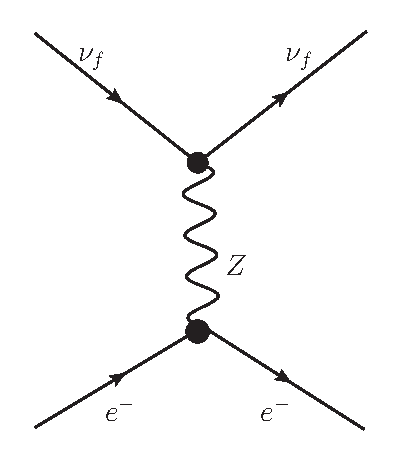
\includegraphics[height=4cm]{neutral.eps}
\end{minipage}
	\caption{Feynman diagrams (at tree level) for different channels of the elastic scattering interaction. (a) and (b): charged current for s and t channels, respectively; (c): neutral current.}
	\label{feynman-es}
\end{figure}


\subsection{Atmospheric Neutrino}
Cosmic rays from outer space continuously interact with nuclei in the atmosphere and produce secondary particles. Atmospheric neutrinos come from decay products of the hadrons in the secondaries. The dominant processes of atmospheric $\nu_e$ and $\nu_\mu$ production is $\pi^+\to\mu^+ + \nu_\mu$ followed by $\mu^+ \to e^+ + \bar{\nu}_\mu + \nu_e$. In the 1980s, the Kamiokande experiment in Japan measured atmospheric neutrinos by utilizing a 3-kiloton water-Cherenkov detector. The incoming neutrinos, $\nu_e$ ($\nu_\mu$) interacted with the water via charged current interactions and electrons (muons) were produced. The electrically charged leptons traversed the water at a speed higher than the speed of light in water and thus emit Cherenkov light, which was recorded by the detector as ring patterns (called Cherenkov rings). The produced electrons caused electro-magnetic showers during their propagation in the water while the produced muons propagated almost in straight lines without producing electro-magnetic showers. Then the $\nu_\mu$ (the $\mu$-like events) were separated from the $\nu_e$ (the $e$-like events) by the fact that the $\mu$-like events created sharper Cherenkov rings than the $e$-like events. Kamiokande measured the ratio of fluxes $\Phi(\nu_\mu+\bar{\nu}_\mu)/\Phi(\nu_e+\bar{\nu}_e)$. The fluxes of atmospheric neutrinos are well understood and the ratio $\nu_\mu/\nu_e$ is expected to be $\sim$2 at low energies $\leq$1~GeV. In 1988, they found a deficit of measured $\mu$-like events compared to the prediction. This was later confirmed by IMB in 1992\cite{becker1992electron} and Soudan-2 in 1997\cite{allison1997measurement} and called ``atmospheric neutrino anomaly''\cite{kajita2012atmospheric}.

\section{Neutrino Flavor Transformation}
Neutrino flavor transformation is a quantum mechanical interference phenomenon\cite{akhmedov2019quantum}. It was first discovered in 1998, based on the analysis of atmospheric neutrino fluxes measured by the Super-Kamiokande (SuperK) experiment to solve the ``atmospheric neutrino anomaly'' mentioned in the last section\cite{fukuda1998evidence}. It is the first direct evidence showing that neutrinos have finite masses and the Standard Model (SM) is incomplete.

Based on current knowledge, neutrinos only interact via the weak force and gravity. A neutrino $\nu_\alpha$ is generated with a definite flavor from weak interaction and is related to a charged lepton with a given flavor: the electron ($e$), the muon ($\mu$) or the tauon ($\tau$) and thus $\alpha=e,\mu,\tau$.

\subsection{Vacuum Oscillation}\label{sectVacuumOsci}
For neutrino flavor oscillation experiments, neutrinos are detected in certain flavor eigenstates via weak interaction. A neutrino flavor state vector can be taken as a linear superposition of the mass eigenstates. For three-flavor neutrino mixing, we have\cite{pdg2018}:
\begin{equation}\label{eq:mixingmatrix}
|\nu_f\rangle = \sum_{i=1}^3U^*_{fi}|\nu_i\rangle, 
\end{equation}
where $f=e,\mu,\tau$ and $k=1,2,3$. The unitary PMNS matrix, $U_{PMNS}$, can be parameterized as\footnote{Here we ignore the Majorana CP violation phases, which are cancelled out when tackling with the flavor transformation probability. We will come to this part in section.~\ref{sectMajorana}}: 
\begin{equation}\label{eq:uPMNS}
U_{PMNS} =
\begin{pmatrix}
1 &0 &0\\
0 &\cos\theta_{23} &\sin\theta_{23}\\
0 &-\sin\theta_{23} &\cos\theta_{23}\\ 
\end{pmatrix}
\begin{pmatrix}
\cos\theta_{13} &0 &e^{-i\delta_{CP}}\sin\theta_{13}\\
0 &1 &0\\
e^{-i\delta_{CP}}\sin\theta_{13} &0 &\cos\theta_{13}\\ 
\end{pmatrix}
\begin{pmatrix}
\cos\theta_{12} &\sin\theta_{12} &0\\
-\sin\theta_{12} &\cos\theta_{12} &0\\
0 &0 &1\\ 
\end{pmatrix}.
\end{equation}

In the PMNS matrix, we have four parameters: the three mixing angles $\theta_{12}$, $\theta_{13}$, $\theta_{23}$ and the charge-parity (CP) violation parameter of lepton sector, $\delta_{CP}$. The unknown value of $\delta_{CP}$ is related to leptogenesis, the hypothetical physical process that produced an asymmetry between leptons and anti-leptons in the very early universe\cite{wiki_cp}. 

Now discuss the vacuum flavor oscillation: in the lab frame, assume a neutrino is generated at time $t_0=0$ from a source with a certain flavor state $|\nu_\alpha\rangle$. It then propagates in vacuum with a speed close to the speed of light (ultra-relativistic) for a distance $L$ and is finally detected at time $t$ in a detector. The flavor eigenstate evolves in space-time is $|\nu_\alpha \rangle = \sum_i U^*_{\alpha i}|\nu_i,p_i\rangle$, where $p_i$ is the 4-momentum of $\nu_i$. The momentum is assumed to be along the direction from the source to the detector and only in one dimension. Via the Schr\"{o}dinger equation, the amplitude for the flavor eigenstate $|\nu_\beta>$ in the detector at $(L,t)$ is (use the natural units: $\hbar=c=1$) \cite{aitchison2012gauge}:
\begin{equation}
\mathcal{A}(\nu_\alpha\to\nu_\beta;L,E)=\sum_{i}U^*_{\alpha i}e^{-iE_i t+ip_iL}\langle\nu_\beta|\nu_i,p_i\rangle=\sum_{i}U^*_{\alpha i}U_{\beta i}e^{-iE_it+ip_iL},
\end{equation}

Then the probability of $\nu_\alpha$ at time $t_0=0$ transforms into a $\nu_\beta$ at time $t$ is:
\begin{equation}\label{oscillationEq1}
 \begin{split}
&P(\nu_\alpha\to\nu_\beta;L,E)=|\langle\mathcal{A}(\nu_\alpha\to\nu_\beta;L,E)|\mathcal{A}(\nu_\alpha\to\nu_\beta;L,E)\rangle|^2=\\
&(U^*_{\alpha 1}U_{\beta 1}e^{-iE_1t+ip_1L}+U^*_{\alpha 2}U_{\beta 2}e^{-iE_2t+ip_2L}+...)(U_{\alpha 1}U^*_{\beta 1}e^{+iE_1t-ip_1L}+U_{\alpha 2}U^*_{\beta 2}e^{+iE_2t-ip_2L}+...)=\\
&\sum_i |U_{\alpha i}|^2|U_{\beta i}|^2 + \sum_{i>j}(U^*_{\alpha i}U_{\beta i}U_{\alpha j}U^*_{\beta j})\exp\{-i(E_i-E_j)t+i(p_i-p_j)L\}+(i\leftrightarrow j),
\end{split}
\end{equation}
where $(i\leftrightarrow j)$ stands for the second term exchanging the $i,j$ indices.

For the second term in \ref{oscillationEq1}: in the ultra-relativistic case, $p_i\simeq p_j\equiv p\simeq E\gg m$, where $E$ is the average energy. Then $E_i=\sqrt{p^2_i+m^2_i}\simeq p+\frac{m_i^2}{2E}$ and thus $E_i-E_j\simeq \frac{m^2_i-m^2_j}{2E}\equiv \frac{\Delta m^2_{ij}}{2E}$\cite{pdg2018,aitchison2012gauge}. Here $\Delta m^2_{ij}$ is a set of parameters called mass square difference, popping out in the flavor transition probability. Along with $L\simeq ct=t~(c\equiv 1)$, we have $\exp\{-i(E_i-E_j)t+i(p_i-p_j)L\}\simeq \exp\{-i\frac{\Delta m^2_{ij}}{2E}\}$. In addition, $U^*_{\alpha i}U_{\beta i}U_{\alpha j}U^*_{\beta j}=|U^*_{\alpha i}U_{\beta i}U_{\alpha j}U^*_{\beta j}|\exp\{i\phi_{\alpha\beta;ij}\}$, where $\phi_{\alpha\beta;ij}=\mathrm{Arg}(U^*_{\alpha i}U_{\beta i}U_{\alpha j}U^*_{\beta j})$ and $\phi_{\alpha\beta;ij}=-\phi_{\alpha\beta;ji}$. Then combine the second term and the $(i\leftrightarrow j)$ term, \ref{oscillationEq1} can be written as\cite{aitchison2012gauge}:
\begin{equation}\label{oscillationEq2}
P_{\nu_\alpha\to\nu_\beta}(L,E)=
\sum_i |U_{\alpha i}|^2|U_{\beta i}|^2 + 2\sum_{i>j}|U^*_{\alpha i}U_{\beta i}U_{\alpha j}U^*_{\beta j}|\cos(\frac{\Delta m^2_{ij}}{2E}L-\phi_{\alpha\beta;ij}).
\end{equation}

Further expand the second term in \ref{oscillationEq2}:
\begin{equation}
 \begin{split}
&|U^*_{\alpha i}U_{\beta i}U_{\alpha j}U^*_{\beta j}|\{\cos(\phi_{\alpha\beta;ij})\cos(\frac{\Delta m^2_{ij}}{2E}L)+\sin(\phi_{\alpha\beta;ij})\sin(\frac{\Delta m^2_{ij}}{2E}L)\}=\\
&\Re(U^*_{\alpha i}U_{\beta i}U_{\alpha j}U^*_{\beta j})(1-2\sin^2\frac{\Delta m^2_{ij}L}{4E})+\Im(U^*_{\alpha i}U_{\beta i}U_{\alpha j}U^*_{\beta j})\sin\frac{\Delta m^2_{ij}L}{2E},
 \end{split}
\end{equation}

since the matrix $U$ is unitary and when $t=0$, 
\begin{equation}
P_{\nu_\alpha\to\nu_\beta}=\delta_{\alpha\beta}=\sum_i |U_{\alpha i}|^2|U_{\beta i}|^2+2\sum_{i>j}\Re(U^*_{\alpha i}U_{\beta i}U_{\alpha j}U^*_{\beta j}),
\end{equation} 

finally it comes out the commonly used vacuum oscillation equation\cite{pdg2018,aitchison2012gauge}:
\begin{equation}\label{common_oscillation}
P_{\nu_\alpha\to\nu_\beta}(L,E)=\delta_{\alpha\beta}-4\sum_{i>j} \Re[U_{\beta i}U^*_{\alpha i}U_{\alpha j}U^*_{\beta j}]\sin^2\frac{\Delta m^2_{ij}L}{4E}+2\sum_{i>j} \Im(U_{\beta i}U^*_{\alpha i}U_{\alpha j}U^*_{\beta j})\sin\frac{\Delta m^2_{ij}L}{2E}.
\end{equation}

Choose a set of units commonly used by experiments and with dimensional transformation, we have\cite{pdg2018}:
\begin{equation}
X_{ij}\equiv \frac{\Delta m^2_{ij}L}{4E}=\frac{1.267\Delta m_{ij}^2[eV^2]L[m]}{E_\nu[MeV]}.
\end{equation}

Maximum oscillation occurs when $X_{ij}\sim \pi$, which gives an effective length $L^{osc}(\Delta m_{ij},E_\nu)=4\pi E/|\Delta m_{ij}^2|$.

Currently, the four parameters in PMNS matrix as well as the parameters of the $\Delta m_{ij}$ have been measured by neutrino oscillation experiments. These experiments can be classified by the neutrino sources they use. They are the solar, the reactor, the atmospheric, the accelerator and the astronomical and cosmological neutrino experiments. Table~\ref{nu_exp} lists the energy scale of the neutrino source as well as the example experiments.

\begin{table}[ht]
	\caption{\label{nu_exp} Oscillation neutrino experiments.}	
	{\centering
		\begin{tabular*}{135mm}{c@{\extracolsep{\fill}}cccc}
			\toprule 
			type & source & $E_\nu$ & example\\
			\midrule
			solar& the Sun & MeV scale & SNO \\
			reactor& reactor & MeV scale & DayaBay \\
			atmospheric& cosmic-ray& GeV scale & SuperK\\
			accelerator&  $\nu$ beam from accelerator & GeV scale & T2K\\	
			astronomical& astronomical objects & GeV-EeV scale & IceCube\\	
			\bottomrule	
		\end{tabular*}
	}
\end{table}

For the $\Delta m^2_{21}$ and $\theta_{12}$, the combined analysis of the measurements from the reactor experiment KamLAND and SNO gave $\Delta m^2_{21} = 7.59^{+0.21}_{-0.21}\times 10^{-5}eV^2$ and $\tan^2{\theta}_{21}=0.47^{+0.06}_{-0.05}$\cite{abe2008precision}.

The accelerator neutrino experiments as well as the atmospheric neutrino experiments have measured $\Delta m^2_{32}$ and $\theta_{23}$. The most recent results from SuperK show that in NH, $\sin^2\theta_{23}=0.588^{+0.031}_{-0.064}$ and $\Delta m^2_{32} = 2.5^{+0.13}_{-0.20}\times 10^{-3} eV^2$\cite{abe2018atmospheric}. 

In 2012, the reactor neutrino experiment Daya Bay reported the discovery of non-zero $\theta_{13}$ with a significance of 5.2$\sigma$. In 2016, Daya Bay reported that $\sin^2 2\theta_{13} = 0.0841\pm0.0027(stat.)\pm0.0019(syst.)$. This high-precision result makes $\sin^2 2\theta_{13}$ the best measured mixing angle\cite{an2017measurement,qian2019physics}.

In addition, there are two squared-mass differences, $\Delta m^2_{21}=m_2^2-m_1^2$ and $\Delta m^2_{32}=|m_3^2-m_2^2|$. The sign of $\Delta m^2_{32}$ is unknown and it indicates a mass hierarchy problem of whether neutrino mass is normal hierarchy (NH, $m_3>m_2>m_1$) or inverted hierarchy (IH, $m_3<m_1<m_2$)\cite{pdg2018}. 


$L/L^{osc}(\Delta m_{31},E_\nu)\sim 1$ and $L/L^{osc}(\Delta m_{21},E_\nu)\ll 1$
\begin{equation}
P_{\nu_\alpha \to \nu_\beta}(L,E)\simeq \delta_{\alpha\beta}-4|U_{\alpha3}|^3(\delta_{\alpha\beta}-|U_{\beta 3}|^2)\sin^2\frac{\Delta m^2_{31}L}{4E}=P_{\bar{\nu}_\alpha \to \bar{\nu}_\beta}(L,E)
\end{equation}




In the case of antineutrino flavor oscillation, we have: $|\bar{\nu}_\alpha>=\sum_i U_{\alpha i}|\bar{\nu}_i,p_i>$, via the same calculation, a similar oscillation probability equation can be found but with the last term in \ref{common_oscillation} being negative\cite{aitchison2012gauge}:
\begin{equation}\label{antiNu_eq1}
P_{\bar{\nu}_\alpha\to\bar{\nu}_\beta}(L,E)=\delta_{\alpha\beta}-4\sum_{i>j} \Re[U_{\beta i}U^*_{\alpha i}U_{\alpha j}U^*_{\beta j}]\sin^2\frac{\Delta m^2_{ij}L}{4E}-2\sum_{i>j} \Im(U_{\beta i}U^*_{\alpha i}U_{\alpha j}U^*_{\beta j})\sin\frac{\Delta m^2_{ij}L}{2E}.
\end{equation}

This provides a measure of CP violation\cite{aitchison2012gauge}:
\begin{equation}\label{cpV_eq1}
%\begin{split}
\mathcal{A}_{CP}=P_{\nu_\alpha\to\nu_\beta}(L,E)-P_{\bar{\nu}_\alpha\to\bar{\nu}_\beta}(L,E)=
4\sum_{i>j} \Im(U_{\beta i}U^*_{\alpha i}U_{\alpha j}U^*_{\beta j})\sin\frac{\Delta m^2_{ij}L}{2E}.
%\end{split}
\end{equation}

\cite{antonio2018state}

$\delta_{CP}$ is examined by the experiments which measure the difference between neutrino and antineutrino oscillation probabilities $P(\bar{\nu}_\alpha\to\bar{\nu}_\beta)$ and $P(\nu_\alpha\to\nu_\beta)$\cite{xing2011neutrinos}. In 2017, the Tokai-to-Kamioka (T2K) experiment in Japan rejected the hypothesis that neutrinos and antineutrinos oscillate with the same probability at 95\% confidence (2$\sigma$) level. This indicates a hint of CP symmetry broken by neutrinos\cite{abe2017measurement}. In 2019, T2K  claimed confidence intervals for $\delta_{CP}$ with three standard deviations ($3\sigma$): [-3.41,-0.03] for NH and [-2.54,-0.32] for IH. This result indicates that the CP violation exists in leptons\cite{abe2019constraint}.

%\subsection{Atmosphere-accelerator Experiments}
%
%\subsection{Astrophysics Experiments}
%Neutrino telescopes
%Ice cube
%Baikal 


\subsection{Matter Effect}

The matter effect is caused by neutrinos interacting with ambient electrons and nucleons in matter such as the Sun or the Earth. $\nu_e$ interacts with electrons via both charged weak current (exchanging $W$ boson) and neutral weak current ($Z$ boson) while $\nu_\mu$ and $\nu_\tau$ interact only by the neutral current. The $\nu_e$ energy has an addition term, $V_{CC} =\sqrt2G_Fn_e$, where $n_e$ is the number density of the electrons in matter and $G_F$ is the Fermi coupling constant for the weak interaction. This affects the oscillation probabilities for neutrinos propagating in matter compared to vacuum, which is called the Mikheyev-Smirnov-Wolfenstein (MSW) mechanism\cite{smirnov2016solar,smirnov2005msw}.

In vacuum two-flavor mixing, the Schr\"{o}dinger equation can be written (in natural units)\cite{xing2011neutrinos}:
\begin{equation}\label{eq:2flavor_simple}
	i\frac{d}{dt}\begin{pmatrix}
		\nu_e\\
		\nu_\mu\\
	\end{pmatrix}
	=
	H^f_0
	\begin{pmatrix}
		\nu_e\\
		\nu_\mu\\
	\end{pmatrix},
\end{equation}
where 

\begin{equation} \label{eq:H0f}
\begin{aligned}
 H^f_0 = \frac{1}{2E}\begin{pmatrix}m^2_1\cos^2\theta+m^2_2\sin^2\theta & (m^2_2-m^2_1)\sin\theta\cos\theta \\ (m^2_2-m^2_1)\sin\theta\cos\theta & m^2_1\sin2\theta+m^2_2\cos^2\theta\end{pmatrix} =
\\
\frac{\Delta m_{21}^2}{4E}\begin{pmatrix}
	-\cos 2\theta & \sin 2\theta\\
	\sin 2\theta & \cos 2\theta\\
\end{pmatrix}+\frac{(m_1^2+m_2^2)}{4E}\begin{pmatrix}
	1 & 0\\
	0 &1\\
\end{pmatrix},
\end{aligned}
\end{equation}
and $\Delta m^2_{21}=(m^2_2 - m^2_1)$.

To simplify the calculation, we can drop the second unitary term of $H^f_0$ that is irrelevant to the neutrino flavor transformation. Including the matter effect, we obtain:
\begin{equation}\label{eq:Hm}
	H_m = \begin{pmatrix}
		-\frac{\Delta m_{21}^2}{4E}\cos 2\theta+\sqrt 2G_Fn_e & \frac{\Delta m_{21}^2}{4E}\sin 2\theta\\
		\frac{\Delta m_{21}^2}{4E}\sin 2\theta &\frac{\Delta m_{21}^2}{4E}\cos 2\theta\\
	\end{pmatrix}
\end{equation}

We define a mixing angle in matter, $\theta_m$ as:
\begin{equation}\label{eq:thetaM}
	\tan 2\theta_m = \frac{\Delta m^2\sin2\theta}{\Delta m^2\cos2\theta-2\sqrt 2E G_Fn_e},
\end{equation}
and define an effective squared-mass difference in matter $\Delta m^2_m$ as:
\begin{equation}
	\Delta m^2_m = \sqrt{(\Delta m^2\cos2\theta - 2\sqrt 2EG_Fn_e)^2+(\Delta m^2\sin2\theta)^2}.
\end{equation}

In analogy with mixing in vacuum, we can write the mixing equation relating the energy eigenstates in matter ($\nu_{1m},\nu_{2m}$) to the flavor eigenstates with a diagonalized Hamiltonian:
\begin{equation}\label{eq:matter_mixing}
	\begin{pmatrix}
		\nu_e\\
		\nu_\mu\\
	\end{pmatrix}
	= \begin{pmatrix}
		\cos\theta_m & \sin\theta_m\\
		-\sin\theta_m & \cos\theta_m \\
	\end{pmatrix}
	\begin{pmatrix}
		\nu_{1m}\\
		\nu_{2m}\\
	\end{pmatrix}.
\end{equation}

The probability of flavor transformation in matter is:
\begin{equation}
	P_{\nu_e\to\nu_{\mu}}=\sin^2(2\theta_m)\sin^2\Big(\frac{\Delta m_m^2L}{4E}\Big).
\end{equation}

The denominator in equation (\ref{eq:thetaM}) implies a resonance condition:
\begin{equation}\label{eq:reson_condition}
	V(n_e)=\sqrt 2G_Fn_e=\frac{\Delta m^2\cos2\theta}{2E}.
\end{equation}

From this condition, for a given $E$, there is a resonance density $n^{reson}_e$ while for a given $n_e$, there is a resonance energy $E^{reson}$. When the resonance condition is satisfied, $\theta_m = \frac{\pi}{4}$ and two flavor neutrinos are maximally mixed, even if the vacuum mixing angle $\theta$ is small. This is called matter enhanced neutrino oscillation\cite{smirnov2016solar,fukugita2013physics}.

The oscillation probability in matter can be written in a concise and exact form as \cite{kimura2002exact}:
\[
P(\nu_e\to\nu_\mu) = A\cos\delta+B\sin\delta+C
\]

will also provide the information for the CP- and T-violation
by investigating the quantities of:
\[
A_{CP} = \frac{P(\nu_\alpha\to\nu_\beta)-P(\bar{\nu}_\alpha\to\bar{\nu}_\beta)}{P(\nu_\alpha\to\nu_\beta)+P(\bar{\nu}_\alpha\to\bar{\nu}_\beta)}
\]

\[
A_T = \frac{P(\nu_\alpha\to\nu_\beta)-P(\bar{\nu}_\beta\to\bar{\nu}_\alpha)}{P(\nu_\alpha\to\nu_\beta)+P(\bar{\nu}_\beta\to\bar{\nu}_\alpha)}
\]

\subsection{Status of the Neutrino Flavor Transformation Experiments}

Since neutrinos' extremely low interaction cross-sections, neutrinos produced in the Sun can reach the detectors on the Earth without being interrupted. This enables the solar neutrino to be a probe to the stellar physics.

KamLand

Daya Bay

The Jiangmen Underground Neutrino Observatory (JUNO) is a reactor neutrino experiment located at Kaiping, Jiangmen in Southern China. a large liquid scintillator detector 
large active mass of 20 kton

the energy resolution (3\% at 1 MeV) 
\cite{giaz2018status}

\section{Neutrino Mass}\label{sectMajorana}
A free spin-1/2 fermion field with a mass $m$ follows the Dirac equation $(i\gamma^\mu\partial_\mu-m)\psi=0$, where $\partial_\mu\equiv \partial/\partial x^\mu$, $\psi$ is a four-component spinor (Dirac spinor) field, and $\gamma^\mu~(\mu=0,1,2,3)$ is a set of $4\times 4$ matrices forming a Clifford algebra, i.e, satisfying the following relations\cite{akhmedov2014majorana,zee2010quantum}:
\begin{equation}\label{eq:clifford}
\{\gamma^\mu,\gamma^\nu\}=2\eta^{\mu\nu}, 
\end{equation}
where $\eta^{\mu\nu}=diag(1,-1,-1,-1)$ is the Minkowski metric. From \ref{eq:clifford} we can deduce $(\gamma^0)^2=+1$, $(\gamma^i)^2=-1~(i=1,2,3)$ and $\gamma^0\gamma^{\mu\dag}\gamma^0=\gamma^\mu$. The product of four gamma matrices is defined as $\gamma_5\equiv i\gamma^0\gamma^1\gamma^2\gamma^3$, which satisfies $\{\gamma_5,\gamma^\mu\}=0$ and $(\gamma_5)^2=1$. From $\gamma_5$, we can define the left-handed and right-handed chirality projector operators: $P_L\equiv\frac{1}{2}(1-\gamma_5)$ and $P_R\equiv\frac{1}{2}(1+\gamma_5)$.

For fast moving particles, it's convenient to take $\gamma$ matrices in chiral or Weyl representation (in which $\gamma_5$ is diagonal) as\cite{zee2010quantum}:
\begin{equation}
\gamma^0 = \begin{pmatrix} 
0 & I \\
I & 0
\end{pmatrix},
\gamma^i = \begin{pmatrix} 
0 & \sigma^i \\
-\sigma^i & 0
\end{pmatrix},
\gamma_5 = \begin{pmatrix} 
-I & 0 \\
0 & I
\end{pmatrix},
\end{equation}
where $\sigma^i~(i=1,2,3)$ are $2\times 2$ Pauli matrices and $I$ is a $2\times 2$ identity matrix.

The Lagrangian density constructed from the Dirac equation is $\mathcal{L}_D = \bar\psi(i\gamma^\mu\partial_\mu-m)\psi$, where $\bar{\psi}\equiv \psi^{\dag}\gamma^0$ is a adjoint field. The Dirac spinor field $\psi$ can be decomposed into left and right handed fields: $\psi=\psi_L+\psi_R\equiv P_L\psi+P_R\psi$. With $\overline{\psi_L}\psi_L=\overline{\psi_R}\psi_R=0$ the Dirac Lagrangian density which satisfies the Lorentz invariance and is hermitian can be written as\cite{zee2010quantum}:
\begin{equation}\label{diracLagrange}
\mathcal{L}_D = (\overline{\psi_L} i\gamma^\mu\partial_\mu\psi_L+\overline{{\psi}_R} i\gamma^\mu\partial_\mu\psi_R)-m(\overline{{\psi}_R}\psi_L+\overline{{\psi}_L}\psi_R),
\end{equation} 
where the first two terms on the right hand side are kinetic energy terms with separated chiral components; the last two terms are the Dirac mass term $\mathcal{L}^{D}_{mass}$ with coupled chiral components. For the massive Dirac fields, the left-handed component $\psi_L$ is completely independent of the right-handed $\psi_R$. 

A particle-antiparticle conjugation operator $\hat C$ can associate the $\psi_L$ with the $\psi_R$. It is defined as\cite{akhmedov2014majorana}:
\begin{equation}
\hat C: \psi\to \psi^c=\mathcal{C}\bar\psi^T=\mathcal{C}\gamma^0\psi^*,
\end{equation}
where $\mathcal C$ is the charge conjugation matrix and satisfies the following relations:
\begin{equation}
\mathcal C^{-1}\gamma^\mu\mathcal C=-(\gamma^\mu)^T,~~\mathcal{C}^{-1}\gamma_5\mathcal{C}=(\gamma_5)^T,~~\mathcal{C}^\dagger = \mathcal{C}^{-1}=-\mathcal{C}^*
\end{equation}

In the Weyl representation, $\mathcal{C}=i\gamma^2\gamma^0$, then $\mathcal {C}^2=1$, $(\psi^c)^c=\psi$, $(\psi_L)^c=P_R\psi^c=(\psi^c)_R$ and $(\psi_R)^c=P_L\psi^c=(\psi^c)_L$. Therefore the particle-antiparticle operation $\hat C$ converts the antiparticle of a left-handed field to a particle of right handed and vice versa (both the charge and chirality are changed).

In the SM, neutrinos are the spin-1/2 fermions without carrying electrical charges and they could be ``truly neutral'', i.e., no charge-like quantum number can be used to distinguish a neutrino and an antineutrino, which is one of the reasons why they are special. As a comparison, a neutron is spin-1/2 and chargeless but it carries magnetic moments opposite to an antineutron\cite{akhmedov2014majorana}.

By mathematical aesthetics, Ettore Majorana found a representation which makes all the $\gamma$ matrices be pure imaginary so that the Dirac equation gets rid of complex coefficients\cite{majorana2006symmetric}. Also, the Dirac equation can be switched to the Majorana equation: $i\gamma^\mu\partial_\mu\psi-m\psi^c=0$, which is also satisfies the Lorentz invariance\cite{zee2010quantum}. Since $\psi$ and $\psi^c$ have opposite charges, this equation should describe a neutral fermion\cite{zee2010quantum}. 

Unlike the Dirac case, for the Majorana field $\psi^M$, the $\psi^M_L$ and $\psi^M_R$ are not independent. The right-handed component can be the charge conjugate of the left-handed component (or vice versa): $\psi_R=(\psi_L)^c$\cite{akhmedov2014majorana}. Therefore Majorana field can be written as: $\psi^M=\psi_L^M+\psi_R^M=\psi^M_L+(\psi^M_L)^c=\psi^M_L+((\psi^M)^c)_R$, which immediately gives $(\psi^M)^c=\psi^M$. This equation is called the Majorana condition. The result implies that the particles associated with the Majorana fields, or the Majorana fermions, are their own antiparticles and ``truly neutral''\cite{akhmedov2014majorana}. Also, the Majorana equation preserves the handedness\cite{zee2010quantum}. Since the $\psi^M_L$ and $\psi^M_R$ are not independent and can be constructed by each other, the Majorana spinor $\psi^M$ only has two degrees of freedom compared to the Dirac spinor which has four degrees of freedom. These facts indicate that the Majorana fermion theory is more economical than the Dirac one and it is also tailored for describing neutrinos. It is natural that neutrinos are of Majorana nature.

In the SM, the Majorana fermions are not included. Based on the experimental observations such as the discovery of the parity violation in the $\beta$-decay\cite{wu1957experimental}, the measurement of neutrino helicity\cite{goldhaber1958helicity} and so on, a maximal parity violating $V-A$ theory was built and it only allows the left-handed flavor neutrino fields $\nu_{\alpha L}~(\alpha=e,\mu,\tau)$ (or called ``active'' neutrinos) and right-handed flavor antineutrino fields $\overline{\nu_{\alpha R}}$ involving in the weak interaction. In the theory, the neutrino fields $\nu_\alpha$ and the charged lepton fields $\ell_\alpha$ form the left-handed weak isospin doublets (isodoublets) and the right-handed isosinglets, which belong to the SU(2) group. The isodoublet $\Psi_L = (\nu_{\alpha L}, \ell_{\alpha L})^T$ has weak isospin $I=\frac{1}{2}$ and its third components $I_3=+\pm \frac{1}{2}$ for $\nu_\alpha$ and $I_3=-\frac{1}{2}$ for $\ell_\alpha$; the isosinglet $\Psi_R = (\ell_{\alpha R})$ has $I=0$ and $I_3=0$\cite{aitchison2012gauge, greiner2012theoretical}.

According to the Gell-Mann-Nishijima formula $Q=I_3+\frac{1}{2}Y$, where Q is the electric charge and Y is the hypercharge. For $\Psi_L$, $Y=-1$ and for $\Psi_R$, $Y=-2$. The leptons acquire their masses by coupling to the Higgs fields. To realize this, the Higgs scalar fields also form an isodoublet $\Phi = (\phi^+,\phi^0)^T$ with weak isospin $I=\frac{1}{2}$, where $\phi^+$ is a positively charged complex scalar field with $I_3=\frac{1}{2}$ and $\phi^0$ is a neutrally charged complex scalar field with $I_3=-\frac{1}{2}$. Such a coupling of the fermions to the scalar fields is a typical Yukawa coupling. The Lagrangian of the Yukawa coupling in the lepton sector is\cite{funchal2013physics}:

\begin{equation}\label{yukawa}
-\mathcal L_{Yukawa}(\Phi,\Psi) =\sum_{\alpha,\beta=e,\mu,\tau} y^{lep'}_{\alpha\beta} \overline{\Psi_{\alpha L}'}\Phi\ell_{\beta R}' + h.c.,
\end{equation}
where $y^{lep'}_{\alpha\beta}$ are complex Yukawa coupling matrices of charged leptons and the $h.c.$ means hermitian conjugate. The terms are invariant under the $SU(2)_L\times U(1)_Y$ group transformations required by the SM. The apostrophes indicate that these matrices are not diagonalized.

The lack of the isosinglet term $\nu_R$ in the SM makes neutrino massless. The simplest extension to the SM to create neutrino masses is to introduce the SU(2) singlet states, or the right-handed neutrino fields $\nu_R$. This kind of isosinglet does not participate in the electroweak interactions and are thus called sterile neutrinos. By introducing the $\nu_R$, the SM is minimally extended and neutrinos can be massive\cite{giunti2007fundamentals}.

Since the hypercharge of $\overline{\Psi_{\alpha L}}$ is $Y=+1$ and $\nu_R$ is $Y=0$, the product $\overline{\Psi_{\alpha L}}\nu_{\beta R}$ is $Y=1$. In order to form the $SU(2)_L\times U(1)_Y$ invariant term, a conjugated Higgs doublet with hypercharge $Y=-1$ is built as $\widetilde{\Phi}=i\sigma_2\Phi^*$, where $\sigma_2$ is a Pauli matrix\cite{giunti2007fundamentals}.

Then with right-handed singlets $\nu_R$, \ref{yukawa} turns to be\cite{giunti2007fundamentals,funchal2013physics}:
\begin{equation}\label{yukawa2}
-\mathcal{L}_{Yukawa} =  \sum_{\alpha\beta} y^{lep'}_{\alpha\beta} \overline{\Psi_{\alpha L}'}\Phi\ell_{\beta R} + \sum_{\alpha\beta} y^{\nu'}_{\alpha\beta} \overline{\Psi_{\alpha L}'}\widetilde{\Phi}\nu_{\beta R}'+h.c..
\end{equation}

The Higgs field obtains a vacuum expectation value (VEV) $v_0=\langle\Phi\rangle$ via the electro-weak symmetry breaking process. Taking the unitary gauge, $\Phi=\frac{1}{\sqrt 2}\begin{pmatrix}0\\v_0+h \end{pmatrix}$, where $h$ is a real scalar Higgs field. 

To diagonalize the Lagrangian \ref{yukawa2} to obtain definite masses of the fields, taking the unitary matrices: $V^{lep}_L, V^{lep}_R,V^\nu_L$ and $V^\nu_R$, the Yukawa coupling matrices can be diagonalized by biunitary transformations: $y^{lep}={V^{lep}_L}^\dagger y^{lep'}V^{lep}_R$, with $y^{lep}_{\alpha\beta}=y^{lep}_\alpha\delta_{\alpha\beta}$ for charged leptons; $y^{\nu}={V^{lep}_L}^\dagger y^{\nu'}V^{lep}$, with $y^{\nu}_{\alpha\beta}=y^{\nu}_\alpha\delta_{\alpha\beta}$ for neutrinos. The fields are transformed as: $\ell_{L,R}=({V^{lep}_{L,R}}^\dagger) \ell_{L,R}'$ and
$\nu_{L,R}=({V^\nu_{L,R}}^\dagger)\nu'_{L,R}$, where $\ell_{L,R}'=(e',\mu',\tau')_{L,R}^T$ and ${\nu}_{L,R}'=(\nu_e',\nu_\mu',\nu_{\tau}')_{L,R}^T$ are in the flavor or generation space. The transformed fields $\ell_{L,R}$ and $\nu_{L,R}$ have definite masses. The product ${V_L^{lep}}^\dagger V_L^\nu\equiv U$ is actually the PMNS matrix which has the relation: $\nu_{fL} = \sum_{i=1,2,3}U_{fi}\nu_{iL}$\cite{funchal2013physics,lesgourgues2013neutrino}.

Thus the diagonalized Lagrangian \ref{yukawa2} becomes\cite{funchal2013physics}:

\begin{equation}\label{yukawa3}
-\mathcal{L}_{Yukawa} = (\frac{v_0+h}{\sqrt 2})\sum_{f=e,\mu,\tau}(y_f^{lep})\overline{\ell_{fL}} \ell_{fR}+\sum_{i=1,2,3}(y_i^{\nu})\overline{\nu_{iL}}\nu_{iR}+h.c.,
\end{equation}

In the Lagrangian \ref{yukawa3}, the terms proportional to the VEV of the Higgs doublet are mass terms while the terms proportional to the $h$ describe the couplings between leptons and Higgs boson\cite{giunti2007fundamentals}. If neutrinos are Dirac particles, the mass term in \ref{diracLagrange} is $-\mathcal L_{\nu~mass}^D = m_D\overline{\nu_L}\nu_R+h.c.$. In this case, the Dirac mass term becomes:
\begin{equation}\label{eq:diracMass}
-\mathcal L^D_{mass} =\sum_{\alpha=e,\mu,\tau}\frac{v_0}{\sqrt{2}}(y_\alpha^{lep})\overline{\ell_{\alpha L}}\ell_{\alpha R}+\sum_{i=1,2,3}\frac{v_0}{\sqrt{2}}(y_{i}^\nu)\overline{\nu_{iL}}\nu_{iR}+h.c.,
\end{equation}
So the charged lepton masses are given by: $m_{\ell_\alpha}=\frac{y_\alpha^{lep} v_0}{\sqrt 2}~(\alpha=e,\mu,\tau)$ and the neutrino masses are: $m_i=\frac{y_k^\nu v_0}{\sqrt 2}~(i=1,2,3)$\cite{funchal2013physics}. 

In this Dirac mass case, the masses of charged leptons and neutrinos are both proportional to the Higgs VEV. However, the experimental measurements already show the masses of neutrinos are $\mathcal O(eV)$ 
while charged leptons are $\mathcal O(MeV)$. The smallness of neutrino masses should be obtained by the tuning of the Yukawa couplings $y_k^\nu$, which does not have solid physics meanings or explanations.

If neutrinos are Majorana fermions, since $\nu_L^c=(\nu^c)_R=(\nu)_R$, we can take the neutrino field as $\nu=\nu_L+\nu_L^c$ without introducing the extra $\nu_R$. For simplicity, only considering one flavor generation (such as $\nu_e$), then the Majorana mass term is:  
\begin{equation}\label{major_mass}
\mathcal{L}^{M,L}_{\nu~mass} = -m_L\bar{\nu}\nu=-\frac{1}{2}m_L\overline{\nu_L^c}\nu_L+h.c.,
\end{equation}
where the $1/2$ factor is to avoid double counting of $\nu_L^c$ and $\overline{\nu_L}$ since $\nu_L^c=\mathcal{C}\overline{\nu_L}^T$\cite{giunti2007fundamentals}. For this Majorana mass term, if considering the $U(1)$ group transformations: $\psi\to e^{i\alpha}\psi$ and $\bar \psi \to \bar\psi e^{-i\alpha}$, where $\alpha$ is an arbitrary phase parameter. We find that in the Dirac case, the mass term in the form of $\psi\bar\psi$ is invariant under $U(1)$ transformations while in the Majorana case it is not. This means that the Majorana fields break the conservation of all the $U(1)$ charges, such as the electric charge and lepton number\cite{akhmedov2014majorana}. Since the law of electric charge conservation is solid in our universe, the particle with a Majorana mass must be electrically neutral while on the other hand, the lepton number for the Majorana fermion is not conserved, which is not described in the Standard Model. The neutrinoless double beta decay process discussed in the next section will come back to this point.

Also, since the terms $\overline{\nu_L^c}\nu_L+h.c.$ are with the weak isospin $I_3=1$ and then $Y=-2$, it requires a Higgs triplet with $Y=2$, which is not included in the Standard Model\cite{funchal2013physics}. Therefore, new physics beyond the Standard Model is required for describing the Majorana mass term.

For a more general case: a hybrid mass term of Dirac and Majorana, if only considering one neutrino generation for simplicity, we can write the Dirac mass term in \ref{diracLagrange} as the same form of the Majorana mass term: $\mathcal{L}_{\nu~mass}^D = -\frac{1}{2}m_D(\overline{\nu_L}\nu_R+\overline{\nu^c_R}\nu^c_L)+h.c.$. Likewise, introduce the $\nu_R$ to the Majorana case and then we have a Majorana mass term with right-handed component: $\mathcal{L}^{M,R}_{\nu~mass} = -m\bar{\nu}\nu=-\frac{1}{2}m_R\overline{\nu_R^c}\nu_R+h.c.$. Therefore, the hybrid mass term combining the Majorana and Dirac fields is\cite{akhmedov2014majorana,zuber1998physics}:
\begin{equation}\label{hybridmass}
-\mathcal{L}^{D+M}_{\nu~mass} = -(\mathcal{L}^{D}_{\nu~mass}+\mathcal{L}^{M,L}_{\nu~mass}+\mathcal{L}^{M,R}_{\nu~mass})=\frac{1}{2}N^T_L\mathcal{C}^\dagger
\mathcal{M}N_L+h.c.,
\end{equation}
where $N_L\equiv(\nu_L,(\nu_R)^c)^T=(\nu_L,\mathcal{C}\overline{\nu_R}^T)$; with $m_L$ ($m_R$) for the mass of the left-handed (right-handed) neutrino field, the mass matrix is written as:
\footnote{Here only considering one neutrino generation. In the general case $\mathcal M$ is a $(n_a+n_s)\times(n_a+n_s)$ matrix, for $n_a$ active neutrinos and $n_s$ sterile neutrinos\cite{akhmedov2014majorana,zuber1998physics}.}:
\begin{equation}
\mathcal M=
\begin{pmatrix}
	m_L^M &  m^D\\
	m^D &  m_R^M\\
\end{pmatrix}.
\end{equation}

Using a unitary matrix $U$ to diagonalize the $\mathcal M$ so that ${U}^T\mathcal{M} U =\mathcal {M}_d = \mathrm{diag}(m_1, m_2)$; $m_{1,2}\geq 0$ are the mass eigenvalues of the eigenstates $\nu_{1,2}$ and 
\begin{equation}\label{eq:massTransform}
U=\mathcal{O}\rho=\begin{pmatrix}
\cos\theta & \sin\theta\\
-\sin\theta & \cos\theta\\
\end{pmatrix}\begin{pmatrix}
\rho_1 & 0\\
0 & \rho_2\\
\end{pmatrix},
\end{equation}
where $\mathcal O$ is a real orthodox matrix and $\rho$ is a phase matrix with $(\rho_{1,2})^2=\pm1$ to guarantee that $m_{1,2}\geq 0$.
From the transformation, the off-diagonal elements give a relation of $\theta$: $\tan 2\theta = \frac{2m_D}{m^M_R-m^M_L}$, which indicates a mixing of the normal active Dirac neutrino with a pair of the sterile Majorana neutrinos. For the left-handed neutrino mass eigenstates $\nu_{1L}$ and $\nu_{2L}$, there is\cite{akhmedov2014majorana}:
\begin{equation}\label{eq:NLtransform}
N_L=\begin{pmatrix}
\nu_{L}\\
(\nu_{R})^c\\
\end{pmatrix}=U
\begin{pmatrix}
\nu_{1L}\\
\nu_{2L}\\
\end{pmatrix},
\end{equation}
Define
$\nu_{i}=\nu_{iL}+(\nu_{iL})^c~(i = 1,2)$, the Lagrangian \ref{hybridmass} now can be written as\cite{akhmedov2014majorana,giunti2007fundamentals}:
\begin{equation}
-\mathcal L=\frac{1}{2}N_L^T\mathcal{C}^{\dagger}\mathcal M N_L+h.c.=\frac{1}{2}\nu_L^T\mathcal{C}^{-1}\mathcal M_{diag} \nu_L+h.c.=\frac{1}{2}(|m_1|\overline{\nu_1}\nu_1+|m_2|\overline{\nu_2}\nu_2).
\end{equation}

On the other hand, the mass eigenvalues are solved as:
\begin{equation}
m_{1,2}\equiv m_{\mp} = \frac{1}{2}[~(m_L^M+m_R^M)\mp\sqrt{(m_L^M-m_R^M)^2+4(m^D)^2}~]\label{eq:majorana_massEigen},
\end{equation}

From (\ref{eq:majorana_massEigen}), there are 4 cases to discuss:\\
(1) If $m_L^M=m_R^M=0$ (called ``Dirac limit''), then $m_{1,2}=m^D$ and neutrinos are pure Dirac particles.\\
(2) If $m^D\gg m^M_{L,R}$, then $\tan 2\theta=\frac{2m^D}{m^M_R-m^M_L}\gg 1$ and $\theta\simeq \pi/4$, ${m_{L,R}^M}/{m^D}\to 0$, $m_{1,2}=\frac{1}{2}m^D[~\frac{(m_L^M+m_R^M)}{m^D}+\sqrt{(\frac{m^M_L-m^M_R}{m^D})^2+4}~]\simeq\frac{1}{2}m^D(0+\sqrt{0+4})= m^D$, the pair of Majorana neutrinos behaves like one Dirac neutrino, which is called a Pseudo-(or quasi-)Dirac Neutrino.
\\
(3) If $m^D=0$, $m_1=m^M_L, m_2=m^M_R$, neutrinos are pure Majorana particles.\\
(4) If $m_R^M\gg m^D, m_L^M$, then $\theta\simeq({m^D}/{m_R^M})\ll 1$ and $\tan 2\theta=\frac{2m^D}{m^M_R-m^M_L}\to 0$, we get:
\begin{equation}
\begin{aligned}
m_1=m_-&=\frac{1}{2}\frac{(m^M_L+m^M_R)^2-(m^M_L-m^M_R)^2-4(m^D)^2}{m^M_L+m^M_R+|m^M_L-m^M_R|\sqrt{1+(\frac{2m^D}{m^M_L-m^M_R})^2}}\simeq 
\frac{2m^M_Lm^M_R-2(m^D)^2}{m_L^M+m_R^M+(m_R^M-m_L^M)}\\
&=|m^M_L-{(m^D)^2}/{m^M_R}|,
\end{aligned}
\end{equation}\footnote{Here the absolute value is taken because we can find proper $\rho_{1,2}$ values to ensure $m_1\geq 0$.}
and:
\begin{equation}
m_2=m_+=\frac{1}{2}[m^M_R+m^M_R(1+\frac{1}{2}({2m^D}/{m^M_R})^2)]=m^M_R[1+({m^D}/{m^M_R})^2].
\end{equation}

In the case of (4), since $\theta\ll 1$, $U\simeq \mathrm{diag}(\rho_1, \rho_2)$, from \ref{eq:NLtransform}, the mass eigenstates $\nu_1\simeq \nu_L+(\nu_L)^c, \nu_2\simeq \nu_R+(\nu_R)^c$. Since $\nu_{1,2}=(\nu_{1,2})^c$, it means that the massive neutrino eigenstates are of Majorana nature. It also shows that the mass eigenstate $\nu_2$ relates to the right-handed sterile neutrino $\nu_R$ while the $\nu_1$ relates to the left-handed active neutrino $\nu_L$. Considering $m_L^M = 0$ in the Standard Model\cite{akhmedov2014majorana}, if the sterile neutrino $\nu_R$ is heavy, the mass of the active neutrino $m_1= {(m^D)^2}/{m^M_R}$ will be light. This is called the Seesaw Mechanism. 

In the Seesaw Mechanism, new neutral force carriers or messenger particles with unknown masses $M_x$ are added into the Standard Model. There are mainly three types of Seesaw mechanism, depending on what new particles are introduced.  Generally, a dimension-5 operator $\mathcal{O}_5=\frac{\kappa}{M_X}\Psi_{L}\Psi_{L}\Phi\Phi$ is considered, where $\kappa$ is an unknown dimensionless coupling constant, $\Psi_{L}$ is the $SU(2)_L$ lepton doublet and $\Phi=(\phi^+,\phi^0)^T$ is the Higgs doublet\cite{barger2012physics}. Via symmetry breaking at the electroweak scale ($v_0=246~GeV$), the neutrino mass can be obtained as $m_\nu=\kappa v_0^2/M_X$. In the case (4), adding a neutral, heavy right-handed neutrino $\nu_R$ is called the type-I, or the conventional Seesaw Mechanism; its tree-level Feynman diagram is shown in Fig.~\ref{seesaw} (left).
Since we know the Dirac mass $m^D=y_\nu v_0$ (from \ref{eq:diracMass}), $m_1=y^2_\nu v_0^2/m^M_R$. Since $m^D\propto v_0\sim\mathcal{O}(100~GeV)$, if the active neutrinos is in the mass scale of $m_1\sim\mathcal{O}(0.01~eV)$, then $m^M_R\sim\mathcal{O}(10^{15}~GeV)$, which is a value close to the expected grand unification theory (GUT) mass scale $m_{GUT}~\mathcal{O}10^{16}$. For the type-II, heavy $SU(2)_L$ triplet Higgs scalars $\Delta$ are introduced; its diagram is shown in Fig.~\ref{seesaw} (right). For the type-III, heavy triplet fermions are introduced; its diagram is similar to the type-I, but with different exchanging particles.

\begin{figure}[htbp]
	\centering	
	%	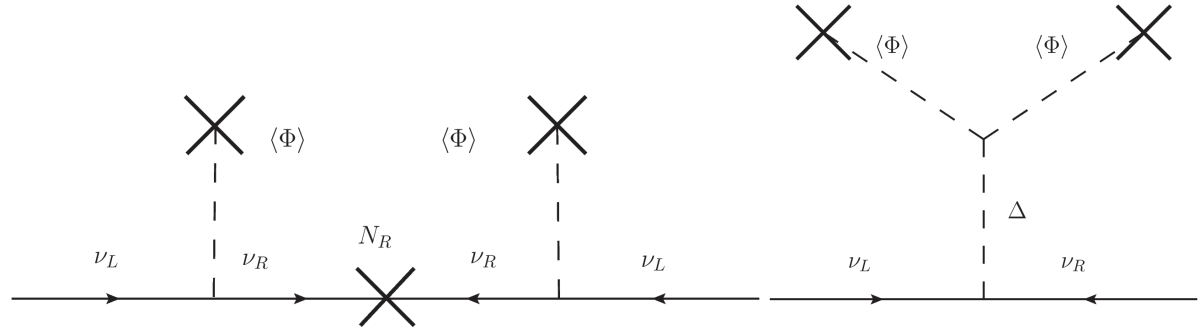
\includegraphics[height=3cm]{seesaw_feynman}
	\begin{minipage}[t]{0.6\textwidth}
		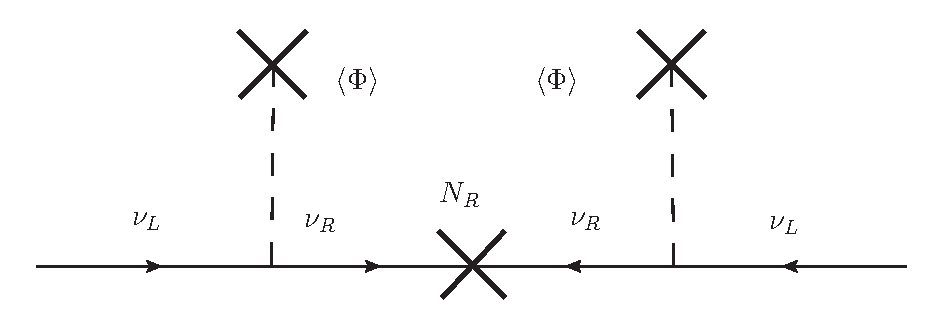
\includegraphics[width=8cm]{typeI_seesaw.eps}
	\end{minipage}
	\begin{minipage}[t]{0.3\textwidth}
		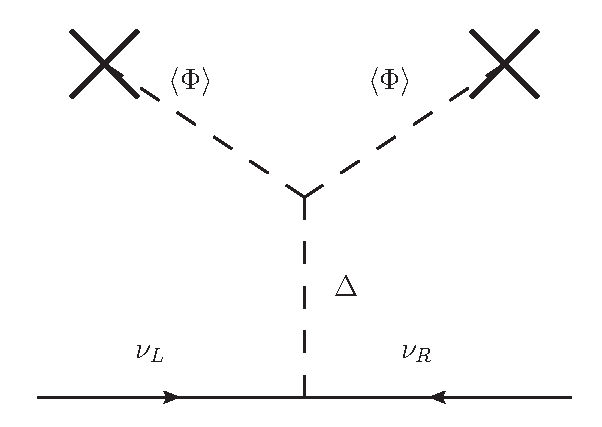
\includegraphics[height=3.0cm]{typeIIseesaw.eps}
	\end{minipage}
	\caption{ Tree-level Feynman diagrams for the Seesaw Mechanisms, modified from \cite{valle2015neutrinos}. Left: type-I; right: type-II. The type-III scheme shares the same diagram to the type-I, but with the $\nu_R$ replaced by $T^0$.}
	\label{seesaw}
\end{figure}

As a summary, to explain how the neutrinos acquire their masses, new physics theories are required to extend the Standard Model. If neutrinos are Majorana particles, the induced Seesaw Mechanism can explain the tiny mass of the active neutrinos naturally. As a bonus, the mass scale required by the Seesaw Mechanism implies the new physics in GUT.

\section{Measure the Absolute Neutrino Mass}

The results from the neutrino flavor transformation experiments proved that neutrinos are not massless and have finite masses. However, in these experiments, the mass differences, rather than the absolute mass values are measured so we can not know the absolute scale of neutrino masses from these results. Currently, there are mainly three approaches to probe the neutrino masses: (1) cosmological measurements; (2) direct measurements for the $\beta$-decay spectrum; (3) a search for the $0\nu\beta\beta$ process\cite{valle2015neutrinos}. 

\subsection{Cosmological Approach}
Neutrinos play an important role in the formation and evolution of the universe. From the hot big bang model, there exists a relic sea of neutrinos forming a Cosmic Neutrino Background (CNB)\cite{lesgourgues2013neutrino}. Though the CNB has not been detected, the massive neutrinos can leave imprints on cosmological observables, such as the anisotropies of the Cosmic Microwave Background (CMB) temperature spectra, the matter power spectrum from the large-scale structure and the Baryon Acoustic Oscillations (BAO)\cite{dvorkin2019neutrino,gerbino2018status}.

Combining the CMB data from the Planck space observatory (updated to 2018 results) with the BAO measurements, a tight 95\% constraint on the sum of the masses of the three active types of neutrinos is obtained as: $\sum m_\nu<0.12~eV$\cite{aghanim2020planck}. Currently the cosmological approaches provide the strongest upper limit of the sum of neutrino masses\cite{dvorkin2019neutrino}. On the other hand, these measurements are strongly model dependent. For example, the measurements based on CMB mainly depend on the Lambda Cold Dark Matter ($\Lambda CDM$) model, which is a standard model of Big Bang cosmology.

\subsection{Direct Kinetic Measurements from Beta Decay}
The classical experiments in history were designed to measure the kinetic energy of the emitted electron from the $\beta^-$-decay: $(Z,A)\to (Z+1,A)+e^-+\overline{\nu_e}$, where A is the mass of the parent nucleus and Z is the atomic or proton number. The energy difference between the initial and final state nuclei is the sum of the emitted electrons $e^-$ (called the $\beta$-electron ) energy $E_e$, the antineutrino $\bar{nu}_e$ energy $E_\nu$ and the nuclear recoil energy $E_R$: $Q=E_e+E_\nu+E_R$. If considering the initial and final nuclei are at rest and $E_R$ is negligible, due to the presence of $E_\nu$, $E_e$ can range from 0 to the maximal energy $E_0=Q$ (called the end-point energy). For the $\beta$-electron with a rest mass $m_e$, the kinetic energy $T_e=E_e-m_e$ (taking the natural unit $\hbar=c=1$) and the momentum $p_e=\sqrt{E^2+2Em_e}$. Then by using the Fermi's Golden Rule, the differential $\beta^-$-decay spectrum of $T_e$ is given by\cite{rottele2019tritium}:
\begin{equation}\label{eq:beta-decay}
\begin{aligned}
\frac{d^2N}{dtdT_e} = \frac{G_F^2\cos^2\theta_C|\mathcal{M}_{nucl}|^2}{2\pi^3} &\cdot F(Z+1,T_e)\cdot(T_e+m_e)\cdot p_e\cdot (E_0-T_e)\\
&
\cdot \sqrt{(E_0-T_e)^2-m^2_{\bar{\nu}_e}}\Theta(E_0-T_e-m_{\bar{\nu}_e}),
\end{aligned}
\end{equation}
where $G_F$ is the Fermi constant; $\theta_C$ is the Cabibbo angle; $\mathcal{M}_{nucl}$ is the nuclear matrix element; $F(Z,E)$ is the Fermi function describing the electromagnetic interaction between the $\beta$-electron and the final-state nucleus; and the Heaviside step function $\Theta$ ensures that a neutrino can only be emitted if enough energy is left for its mass.

In this spectrum, the square of the rest mass $m^2_{\bar{\nu}_e}=\sum_i |U_{ei}|^2 m_i^2$ is the measurement observable. It can be evaluated by measuring the $\beta$-decay event rate and at the endpoint energy the event rate is proportional to $E_0^{}-3$\cite{rottele2019tritium}.

From the view of experimentalists, the tritium $\beta$-decay process: $^3$H$\to^3$He$^+$+$e^-+\bar{\nu}_e$ has a low endpoint energy $E_0=18.57$ keV, a favorable half-life $T_{1/2}=12.32$ years and simple atomic structure. With these experimental advantages, it has been largely investigated since 1947 and has been used as a standard technology for the kinetic measurement\cite{fukugita2013physics}. Among the tritium experiments, the KATRIN (KArlsruhe TRItium Neutrino) experiment is the state-of-the-art one which uses a high energy resolution spectrometer to measure the tritium $\beta$-decay. In 2019, the experiment reported an upper limit of $m_\nu<1.1$ eV with 90\% C.L.. After 5 years of measurement, the experiment is expected to reach the $m_\nu$ sensitivity down to 0.2 eV with 90\% C.L.\cite{aker2019improved}.

\subsection{Double Beta Decay}

For heavy radioactive isotopes (mass $A>70$) with nuclei of even neutron number ($N$) and even proton number ($Z$) (called even-even nucleus), beta decay will lead to an odd-odd nucleus which is less stable. For some such isotopes the beta decay is energetically forbidden. In 1935, Maria Goeppert-Mayer pointed out that they can still decay through a double beta decay process: $(Z,A) \to (Z+2,A)+2e^{-}+2\bar{\nu_e}+Q_{\beta\beta}$, where the $Q_{\beta\beta}$ is the released energy. This is called ordinary double beta decay or $2\nu\beta\beta$, which is allowed by the Standard Model and with a typical half-life $T_{1/2}>10^{19}$ years\cite{povh2008particles,martin2019nuclear}.

If neutrinos are Majorana particles, a process called neutrinoless double beta decay ($0\nu\beta\beta$) will also be expected. The Feynman diagrams of $2\nu\beta\beta$ and $0\nu\beta\beta$ are illustrated in Fig.~\ref{feynman1}.

\begin{figure}[htbp]
	\centering	
	\begin{minipage}[t]{0.45\textwidth}
		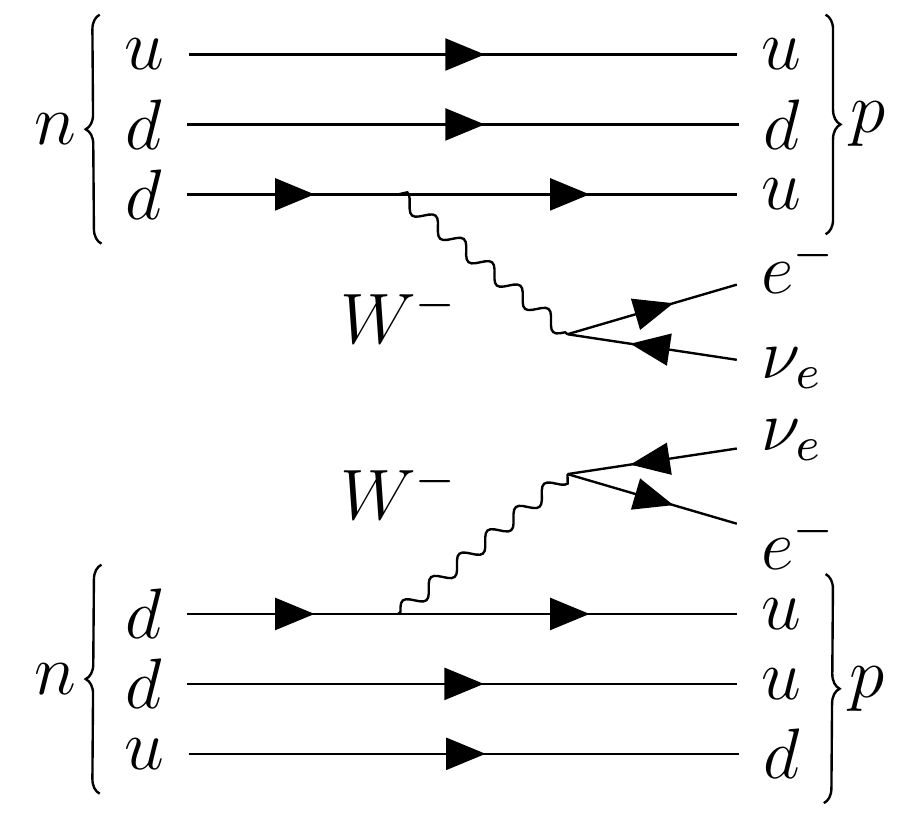
\includegraphics[width=5cm]{doubleBeta2nu_feynman.png}
	\end{minipage}
	\begin{minipage}[t]{0.45\textwidth}
		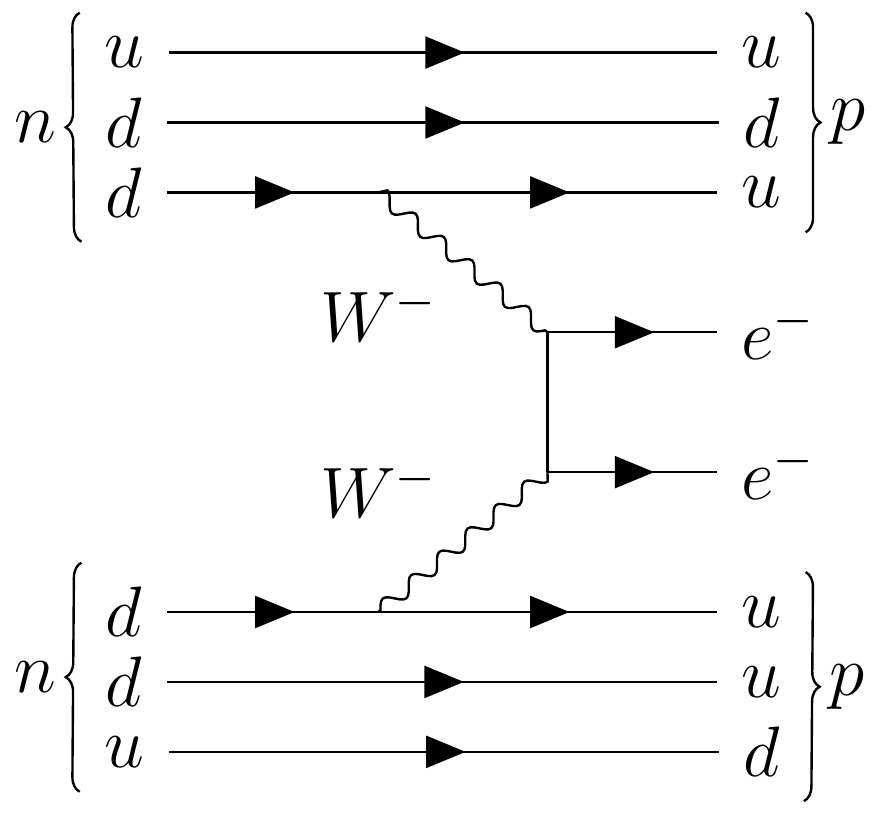
\includegraphics[width=5cm]{doubleBeta_feynman.png}
	\end{minipage}
	\caption{ Feynman diagrams for $2\nu\beta\beta$ (left) and $0\nu\beta\beta$ (right).}
	\label{feynman1}
\end{figure}

\begin{figure}[htbp]
	\centering	
	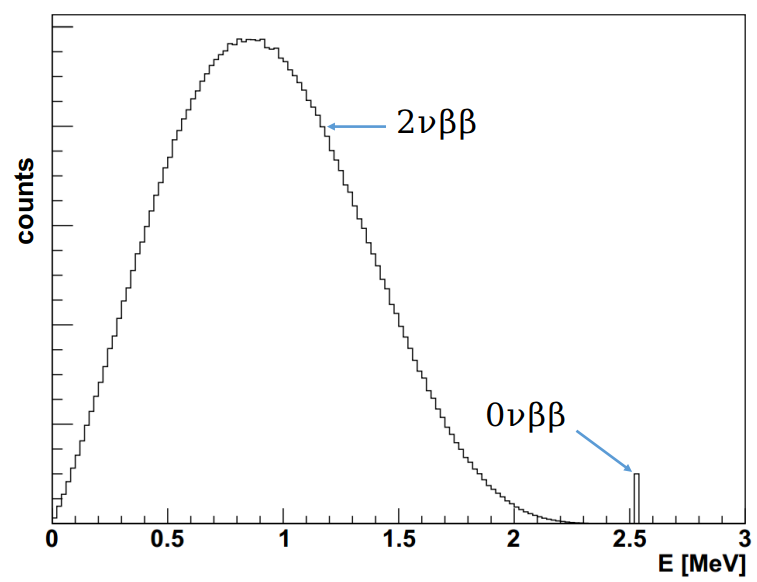
\includegraphics[width=8cm]{Te130_energy0vbb.png}
	\caption{Energy spectrum of the $^{130}$Te $2\nu\beta\beta$ decay and the hypothetical $0\nu\beta\beta$ decay. The SNO+ simulation package (RAT) was used to produce the plot.}
	\label{te130energy}
\end{figure}

The interpretation of the $0\nu\beta\beta$ process is considered as exchanging light Majorana neutrinos. In this case the effective Majorana mass $\langle m_{ee}\rangle=|\sum_{i=1}^{3} U_{ei}^2m_i|~(i=1,2,3)$, $U_{ei}$ are the elements of the neutrino mixing matrix for the flavor state $\nu_e$, and $m_i$ are the mass eigenvalues of the mass eigenstates (from (\ref{eq:mixingmatrix})). The observable quantity is the half-life:
\begin{equation}
(T^{0\nu\beta\beta}_{1/2})^{-1} = G_{PS}(Q,Z)|M_{Nuclear}|^2\langle m_{ee}\rangle^2, 
\end{equation}
where $G_{PS}$ is the phase space factor and $|M_{Nuclear}|$ is the nuclear matrix element for the physics process describing the $0\nu\beta\beta$ decay process\cite{zuber2011neutrino}.

Similar to beta decay, the $2\nu\beta\beta$ process will cause a continuous spectrum in the detector while the $0\nu\beta\beta$ process only has two electrons in the final state, which sum up to give a distinct energy peak. By measuring this exact energy, a detector with high energy resolution is able to search for the $0\nu\beta\beta$ signal from the $0\nu\beta\beta$ decay radioactive isotopes. Diverse technologies have been developed during the past decades. The following section lists some of the mainstream experiments.

\begin{equation}
\langle m_{ee} \rangle = |c^2_{13}c^2_{12}m_1+c^2_{13}s^2_{12}e^{2i\phi_1}m_2+s^2_{13}e^{2i(\phi_2-\delta_{CP})}m_3|
\end{equation}

From the pdg, $\Delta m^2_{21}\simeq 7.4\times 10^{-5}~eV^2,~|\Delta m^2_{31}|\simeq 2.4\times 10^{-3}~eV^2 ,\theta_{12}\simeq 33.8^\circ, \theta_{23}\simeq 48.6^\circ,\theta_{13}\simeq 8.6^\circ, \delta_{CP}\simeq 221^\circ$.

the Schechter-Valle Theorem, or the Black Box theorem.

the standard left-handed interaction


duerr2011quantitative  


A diagram can be drawn as Fig.~\ref{blackbox} for the $0\nu\beta\beta$ process.
In the diagram, two d-quarks are converted into two u-quarks and electrons without emitting neutrinos via some underlying mechanism. Then from crossing symmetry, \cite{akhmedov2014majorana}.

the Black Box theorem relates the effective Majorana neutrino mass with the $0\nu\beta\beta$ amplitude $\langle m_\nu\rangle$, or the Majorana property of the $\nu_e$ with the existence of the $0\nu\beta\beta$ process. 




\begin{figure}[htbp]
	\centering	
	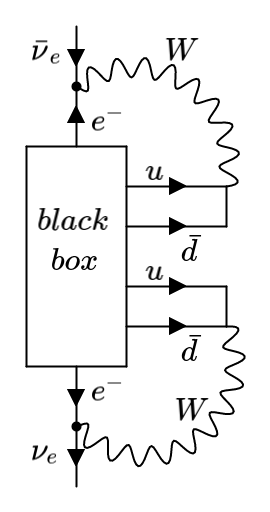
\includegraphics[width=8cm]{blackbox.png}
	\caption{ The Black Box diagram, modified from \cite{schechter1982neutrinoless}.}
	\label{blackbox}
\end{figure}

The Black Box theorem guarantees that if the $0\nu\beta\beta$ process is observed, neutrinos are Majorana particles. An elegant proof was demonstrated by \cite{takasugi1984can} and refined in \cite{duerr2011quantitative,giunti2007fundamentals}. 

\ref{major_mass}.

The phase transformation $\nu_{eL}\to e^{i\eta_{\nu}}|\nu_{eL}\rangle$, where $\eta_\nu$ is a global phase factor.
If this transformation is continuous, then it is actually the global $U(1)$ transformation which implies the conservation of the lepton number. Thus for the $0\nu\beta\beta$ case, $\eta_\nu$ must be discrete and $\eta_\nu\neq 0$. For the other particle fields in the Black Box diagram, there are phase transformations: $e_L\to e^{i\eta_{e}}e_L,~q_L\to e^{i\eta_q}q_L~(q=u,d),~W^\mu_L\to e^{i\eta_W}W_L^\mu$.

the u, d quarks and the electron are massive
the Standard Model left-handed interaction $\bar{\nu}_{eL}\gamma_\mu e_L+\bar{u}_L\gamma_\mu d_L W^\mu$ exists


$\eta_\nu-\eta_e-\eta_W=0$ and $\eta_u-\eta_d-\eta_W=0$.
Combining with these two equations, it gives $\eta_\nu=\eta_d-\eta_u+\eta_e$.


For the $0\nu\beta\beta$ process: $2d\to2u+2e$, the phase transformations give: $\eta_d-\eta_u+\eta_e=0$. Thus $\eta_\nu=\eta_d-\eta_u+\eta_e=0$, which is contradict to the previous condition $\eta_\nu\neq 0$.


violate lepton number by two units and shows that the lepton number is not conserved.

the $\nu_e$ in the $0\nu\beta\beta$ process has a non-zero effective Majorana mass

underlying mechanisms 


\subsection{Status of Double Beta Decay Experiments}

There are 35 isotopes can undergo the double beta decay process, but only a few of them are suitable for the application in direct $0\nu\beta\beta$ search experiments\cite{giunti2007fundamentals}. From the experimental view, the candidate isotopes are expected to have relatively high natural abundances, high Q-values, be deployed in a large amount with low costs, and are not toxic to the environment as well. However, in realistic situation there is no isotope fulfills all these properties and the current experiments making trade-offs\cite{dolinski2019neutrinoless}.

The experiments searching for direct signals of $0\nu\beta\beta$ mainly measure the physics properties of the two emitted electrons, such as their energies, momentum and tracks. 

inhomogeneous experiments use external $\beta\beta$ source
while homogeneous experiments use $\beta\beta$ source as the detection medium, which are mainly referred as calorimeter experiments\cite{cremonesi2014challenges,shimizu2019double}.


$^{136}$Xe, $^{48}$Ca, $^{76}$Ge, $^{130}$Te

At the time of writing, 

$0\nu\beta\beta$ in the range of $10^{25}-10^{26}$ year,



The observed number of event in expectation is: 
\[
N_{event} = \ln 2 \frac{N_A}{M_A}\frac{\alpha\cdot\epsilon\cdot m\cdot t}{T^{0\nu}_{1/2}},
\]

where $N_A$ is the Avogadro's number, $\alpha$ is the abundance of the isotope in the element, 
$M$ is the molar mass of the isotope
and $t$ is the measurement time of total exposure.



The GERmanium Detector Array (GERDA) experiment searches for $0\nu\beta\beta$ of $^{76}$Ge. The experiment uses bare germanium crystals with an enrichment of up to $\sim$87\% $^{76}$Ge operated in a radiopure cryogenic liquid argon (LAr)\cite{agostini2016search}. GERDA Phase I had an exposure of 21.6 kg$\cdot$yr and Phase-II started with 35.6kg from enriched material in December 2015. With combined data of Phase I and Phase II, 

a total exposure of 82.4 kg$\cdot$yr 

In 2017, GERDA reported a 90\% confidence level (C.L.) lower limit for the half-life of $^{76}$Ge, $T^{0\nu}_{1/2}(^{76}$Ge$)>8.0\times 10^{25}$ years.

GERDA reported in 2019 a lower limit half-life of $T^{0\nu}_{1/2}(^{76}$Ge$)>0.9\times 10^{26}$ years at 90\% C.L.\cite{agostini2019probing}. effective $m_{ee}$ is [104,228]~meV.


The Enriched Xenon Observatory (EXO) experiment uses 200-kg liquid Xenon (LXe) time projection chamber (TPC) to search for $0\nu\beta\beta$ in $^{136}$Xe. In 2011 they observed the half life of double beta decay of $^{136}$Xe to be $2.11\times 10^{21}$ years and in 2014 they set a limit on $T^{0\nu}_{1/2}(^{136}$Xe$)>1.1\times 10^{25}$ yr\cite{albert2014search}. EXO is now upgrading to the next 5-tonne experiment (nEXO) and is expected to reach an exclusion sensitivity of $T^{0\nu}_{1/2}(^{136}$Xe) to about $10^{28}$ years at 90\% C.L.\cite{albert2018sensitivity}.

Also looking into $^{136}$Xe, the KamLAND-Zen (ZEroNeutrino) experiment exploits the existing facilities of KamLAND by setting a 3.08-m-diameter spherical inner balloon filled with 13 tons of Xe-loaded liquid scintillator at the center of the KamLAND detector.

liquid scintillator cocktail of 82\% decane and 18\% pseudocumene by volume, 2.7 g/L PPO.

photocathode coverage of 34\%.

Their 2016 results from a 504 kg$\cdot$yr exposure obtained a lower limit for the $0\nu\beta\beta$ decay half-life of $T^{0\nu}_{1/2}(^{136}$Xe$)>1.07\times 10^{26}$ yr at 90\% C.L. and the corresponding upper limits on the effective Majorana neutrino mass are in the range $61-165$ meV\cite{gando2016search}.

The Particle and Astrophysical Xenon Experiment III (PandaX-III) uses a high pressure gas-phase time projection chamber (TPC).

The Cryogenic Underground Observatory for Rare Events (CUORE) experiment searches for $0\nu\beta\beta$ in $^{130}$Te. CUORE is a ton-scale cryogenic bolometer array that arranges 988 tellurium dioxide (TeO$_2$) crystals. CUORE reported first results in 2017 after a total TeO$_2$ exposure of 86.3 kg$\cdot$yr. An effective energy resolution of ($7.7\pm 0.5$) keV FWHM and a background count of ($0.014\pm0.002$) $counts/(keV\cdot kg\cdot yr)$ in the ROI were achieved in that data exposure. Combined with the early data (the data from the two precursor experiments, Cuoricino and CUORE-0), they placed a lower limit of $T^{0\nu}_{1/2}(^{130}$Te$)>1.5\times 10^{25}$ yr at 90\% C.L. and $m_{\beta\beta}<(110-520)$ meV\cite{alduino2018first}. In 5 years live time, the experiment will give a projected sensitivity of $9.5\times 10^{25}$ yr at the 90\% C.L. and set an upper limit on the effective Majorana mass in the range $50-130$ meV\cite{piperno2015dark}.

